\setcounter{chapter}{2}
\chapter{Design of the SOCaaS Solution}
\label{chap:design}

% ========== 3.1 INTRODUCTION ==========
\section{Introduction}
\label{sec:intro}

Design constitutes the decisive step in the materialization of any ambitious technological project. This chapter reveals the rigorous methodology we have adopted to design our SOC-as-a-Service, from the analysis of fundamental requirements to the reasoned selection of key technologies. We present a coherent architecture where each component integrates organically to form a unified security ecosystem, capable of responding to the operational requirements of organizations.

Our approach relies on a systematic comparative analysis of available market tools. We meticulously evaluated potential solutions for each critical SOC functionality---log collection, event correlation, threat detection, and response automation---according to strict technical criteria: performance in high-load environments, interoperability with hybrid infrastructures, regulatory compliance, and cost-effectiveness ratio. This comparative analysis is not limited to a simple juxtaposition of technical characteristics; it integrates practical tests in real-world conditions simulating complex attack scenarios.

The technological choices defended in this chapter result from a deliberate balance between innovation and pragmatism. We favored mature open-source platforms for their flexibility and independence from vendors, while integrating commercial solutions when their operational added value justified the investment. Each retained tool---whether the correlation engine, the orchestration system, or the behavioral analysis modules---is the subject of an in-depth presentation highlighting its specific capabilities, its known limitations, and its adequacy to the use cases identified during our preliminary study.

% ========== 3.2 TOOL SELECTION CRITERIA ==========
\section{Tool Selection Criteria}
\label{sec:criteria}

The choice of technological components for our SOC platform is of paramount importance to guarantee both effective and comprehensive IT security. A careful selection of components enables rapid threat identification, ensures a coordinated response during security incidents, and minimizes financial losses.

\begin{table}[H]
\centering
\caption{Tool Selection Criteria}
\label{tab:criteria}
\renewcommand{\arraystretch}{1.4}
\begin{tabular}{>{\raggedright\arraybackslash}p{3cm} p{10.5cm}}
\toprule
\rowcolor{tableheader}
\textbf{Criterion} & \textbf{Description} \\
\midrule
\textbf{Functionality Coverage} & Capability to identify malicious activities; tools capable of aggregating and analyzing logs; automation and remediation features; monitoring of network, endpoints, cloud, etc. \\
\midrule
\textbf{Integration and Interoperability} & Compatibility with existing ecosystem (SIEM, firewalls, antivirus, etc.); support for standards (Syslog, REST API, common log formats); ability to centralize data (integration with multiple log sources). \\
\midrule
\textbf{Scalability and Performance} & Management of large data volumes without performance loss; adaptability to infrastructure growth (cloud, hybridization); minimal latency for real-time detection and response. \\
\midrule
\textbf{Automation and Orchestration} & Ability to automate repetitive tasks (SOAR playbooks); support for incident response workflows; integration with third-party tools for coordinated response. \\
\midrule
\textbf{Advanced Analysis and Threat Intelligence} & Detection based on Machine Learning and abnormal behavior (UEBA); regular updates of signatures and detection rules; access to Threat Intelligence feeds (MISP, OpenCTI, commercial). \\
\midrule
\textbf{Compliance and Reporting} & Compliance with regulations (GDPR, NIS2, ISO 27001); generation of customizable reports for audits; event history and investigation evidence. \\
\midrule
\textbf{Security and Resilience} & The tool itself must be secure (strong authentication, encryption); high availability and disaster recovery. \\
\midrule
\textbf{Cost and ROI} & Total cost of ownership (licenses, maintenance, infrastructure); pricing model (subscription, penalty based on log volume?); return on investment in terms of reduced detection/response time (MTTD/MTTR). \\
\midrule
\textbf{Support and Community} & Quality of technical support (24/7 for a SOC); clear and regularly updated documentation; active community (open-source tools like Suricata, Zeek, Wazuh). \\
\midrule
\textbf{User Experience and Ease of Use} & Intuitive interface and customizable dashboard; reduction of false positives to avoid alert fatigue; training and support provided by the vendor. \\
\bottomrule
\end{tabular}
\end{table}


% ========== 3.3 KUBERNETES ==========
\section{Kubernetes}
\label{sec:kubernetes}

Kubernetes (K8s) is an open-source platform dedicated to container orchestration, designed to automate the deployment, scaling, and management of containerized applications.

In a Kubernetes cluster, the architecture consists of two main components \cite{k8s-docs}:

\subsection{Kubernetes Components}
\label{subsec:k8s-components}

\begin{enumerate}
    \item \textbf{Control Plane (Master Node):} Manages the overall state of the cluster, maintaining the desired state by continuously comparing the current state with the desired state. The Control Plane itself consists of the following components:
    \begin{itemize}
        \item \textbf{Kube-API Server:} Exposes the Kubernetes API to interact with the cluster.
        \item \textbf{etcd:} Key-value database storing the cluster state.
        \item \textbf{Scheduler:} Assigns Pods to worker nodes based on available resources.
        \item \textbf{Controller Manager:} Monitors and corrects the cluster state.
    \end{itemize}

    \item \textbf{Worker Nodes:} This is where containerized applications run, providing the necessary resources (CPU, memory, storage).
    \begin{itemize}
        \item \textbf{Kubelet:} Ensures pods are functioning, including their containers.
        \item \textbf{kube-proxy:} Maintains network rules on nodes.
        \item \textbf{Container runtime:} Software responsible for running containers (Docker, Containerd, etc.).
    \end{itemize}
\end{enumerate}

\subsection{Main Kubernetes Resources}
\label{subsec:k8s-resources}

\begin{itemize}
    \item \textbf{Pod:} The smallest units, a group of one or more containers, with shared storage and network resources, and a specification on how to run the containers.
    \item \textbf{Deployment:} Defines the lifecycle of pods such as replicas, rolling updates.
    \item \textbf{Service:} Abstraction to expose a set of pods.
    \item \textbf{Ingress:} Manages external HTTP/HTTPS access.
\end{itemize}

We chose Kubernetes to meet our needs for high availability and scalability, and also to benefit from its cloud support. This allows us to create, deploy, and manage modern applications in cloud environments.

\begin{figure}[H]
\centering
\fbox{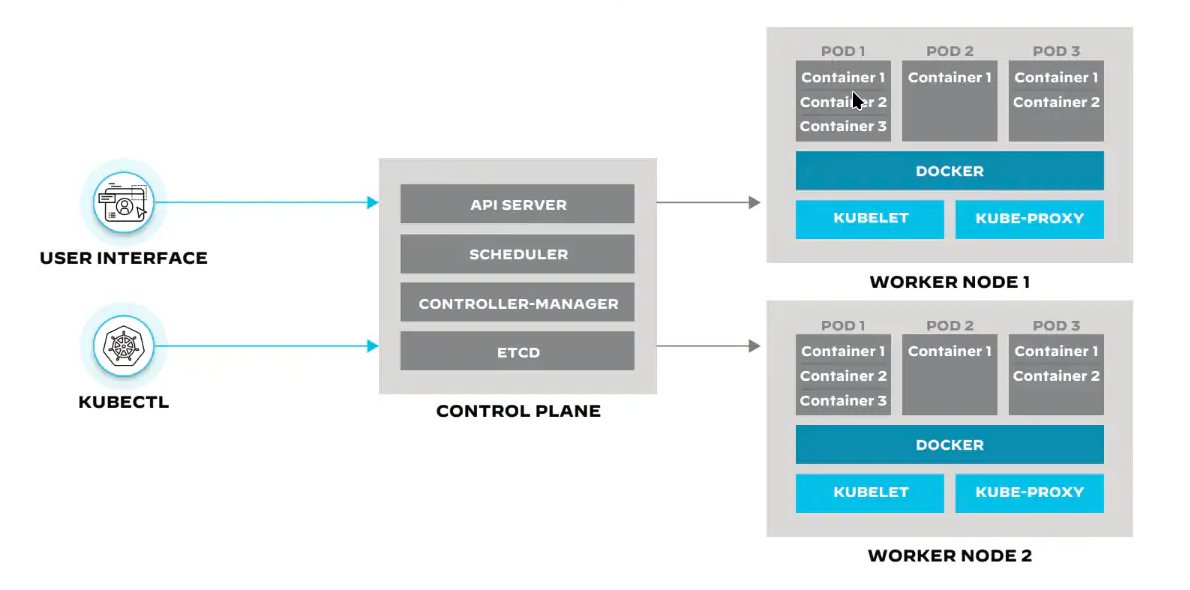
\includegraphics[width=0.9\textwidth]{figs/Kubernetes_Architecture.png}}
\caption{Kubernetes Architecture}
\label{fig:Kubernetes Architecture}
\end{figure}


% ========== 3.4 HELM ==========
\section{Helm}
\label{sec:helm}

Kubernetes represents a valuable tool for cloud developers. Nevertheless, it does not handle all elements on its own: certain issues escape its capabilities or cannot be resolved by Kubernetes \cite{helm-docs}.

Helm is recognized as "the package management tool for Kubernetes," an open-source project initially developed by DeisLabs and now supported by the CNCF. Helm's objective as a package manager is to make the management (installation, update, or uninstallation) of packages for Kubernetes applications simple and automated, and to deploy them with just a few commands \cite{helm-docs}.

\subsection{Key Concepts of Helm}
\label{subsec:helm-concepts}

\begin{enumerate}
    \item \textbf{Charts:} A Helm chart is a ready-to-use package that describes a Kubernetes application. It contains:
    \begin{itemize}
        \item YAML templates: Configuration files for deployments, services, ConfigMaps, etc.
        \item Default values (\texttt{values.yaml}): Customizable parameters such as the number of replicas, CPU/RAM resources.
        \item Metadata (\texttt{Chart.yaml}): File containing chart data such as Name, Version, Description.
    \end{itemize}

    \item \textbf{Release:} A release is an instance of a chart deployed in a Kubernetes cluster. Each release has a unique name and a version history.

    \item \textbf{Repository:} A repository is a remote location that contains and provides these chart packages, such as Artifact Hub.
\end{enumerate}


% ========== 3.5 SIEM CHOICE ==========
\section{SIEM Choice}
\label{sec:siem}

A SIEM constitutes the cornerstone of a modern SOC. It centralizes the collection, analysis, and correlation of security logs. On the market, we find various solutions, whether open-source or proprietary, each designed to meet specific needs.

\subsection{Open-source Solutions}
\label{subsec:siem-open}

\begin{itemize}
    \item \textbf{Wazuh:} Combines SIEM and XDR with vulnerability management and detection while relying on the MITRE ATT\&CK framework rules. Thanks to its unified architecture, it offers seamless integration with various tools.
    \item \textbf{ELK Stack:} Provides log collection, storage, and visualization, offering flexibility through the use of plugins. However, it requires advanced manual configuration.
    \item \textbf{OSSEC:} Focuses on HIDS (Host-based Intrusion Detection System) detection and file monitoring. Lightweight and easy to deploy on endpoints, it nevertheless lacks centralized log management.
\end{itemize}

\subsection{Proprietary Solutions Critical}
\label{subsec:siem-proprietary}

\begin{itemize}
    \item \textbf{Splunk Enterprise Security:} The market leader, benefiting from unparalleled maturity. It offers real-time analysis, AI integration, and advanced reporting. However, its high costs can be a barrier for SMEs.
    \item \textbf{Microsoft Sentinel:} Seamless integration with Azure and SaaS connectors. This system is specially optimized for Microsoft environments and is fully part of the Azure ecosystem.
    \item \textbf{IBM QRadar:} Offers advanced correlation and risk management, accompanied by analytical power adapted to large environments. However, its deployment can be difficult and complex, resulting in high costs.
\end{itemize}

\begin{table}[H]
\centering
\caption{Comparison between Different SIEMs}
\label{tab:siem-compare}
\footnotesize
\setlength{\tabcolsep}{3pt}
\renewcommand{\arraystretch}{1.3}
\begin{tabular}{>{\RaggedRight\arraybackslash}p{2.8cm} >{\RaggedRight\arraybackslash}p{3cm} >{\RaggedRight\arraybackslash}p{3cm} >{\RaggedRight\arraybackslash}p{3cm}}
\toprule
\rowcolor{tableheader}
\textbf{Criterion} & \textbf{Wazuh} & \textbf{IBM QRadar} & \textbf{ELK Stack} \\
\midrule
\textbf{Type} & Open Source & Proprietary & Open Source \\
\midrule
\textbf{Cost} & Free & High cost (licenses, maintenance, support) & Free (possible costs for premium plugins) \\
\midrule
\textbf{Features} & SIEM + XDR + Vulnerability Management & Advanced SIEM + UEBA + Predictive Analysis & Collection, storage, visualization of logs \\
\midrule
\textbf{Threat Detection} & MITRE ATT\&CK rules, correlation based on signatures and behavior & Machine Learning, real-time correlation, risk analysis & Requires manual configurations \\
\midrule
\textbf{Scalability} & Scalable via Kubernetes & High scalability & Horizontal scalability, complex configuration \\
\midrule
\textbf{Integration} & Native with Elastic Stack, Cortex, Kubernetes, MISP & IBM ecosystem, proprietary APIs & Plugins for integration \\
\midrule
\textbf{Threat Intelligence} & Support for MISP, VirusTotal, AbuseDB via Cortex & Integrated TI feeds & Requires external plugins \\
\midrule
\textbf{Compliance} & GDPR, PCI-DSS, NIST modules & Complete certifications & Customizable for compliance, but without predefined modules \\
\midrule
\textbf{Support / Community} & Active community, detailed documentation & Premium IBM support (24/7), but costly & Large community, commercial support \\
\midrule
\textbf{Use Cases} & Ideal for SMEs, SOCaaS, hybrid environments & Large enterprises & Log centralization \\
\bottomrule
\end{tabular}
\end{table}

\subsection{Wazuh}
\label{subsec:wazuh}

Wazuh is a free and open-source security platform that combines XDR (Extended Detection and Response) and SIEM to protect data across different environments. It helps organizations and individuals secure their assets. Wazuh has one of the largest open-source security communities in the world where one can learn, discuss, and contribute \cite{wazuh-community}.

\subsubsection{Wazuh Components}
\label{subsubsec:wazuh-components}

The Wazuh solution relies on the Wazuh agent, deployed on monitored endpoints, and three central components: the Wazuh Server, Wazuh Indexer, and the Wazuh Dashboard.

\paragraph{1. Wazuh Agent \cite{wazuh-agent}}
\label{par:wazuh-agent}

Wazuh Agent is compatible with various operating systems such as Linux, Windows, macOS, Solaris, and AIX. It can be installed on laptops, desktop computers, servers, as well as on cloud instances, containers, or virtual machines. It contributes to protecting your system through:
\begin{itemize}
    \item Threat prevention, detection, and response features.
    \item Application data collection and system log aggregation.
    \item Mutual communication and authentication between agents and server.
\end{itemize}

It contains configurable modules that perform different security tasks and can be activated or deactivated based on specific security needs:
\begin{itemize}
    \item \textbf{Log Collector:} Reads text log files and collects operating system messages.
    \item \textbf{Command Execution:} Executes commands and transmits results to the Wazuh server.
    \item \textbf{File Integrity Monitoring:} Monitors file creation, deletion, or modification.
    \item \textbf{System Inventory:} Performs analyses to collect inventory data.
    \item \textbf{Malware Detection:} This component is capable of detecting anomalies and the possible presence of rootkits.
    \item \textbf{Active Response:} Manages automated actions against threats.
\end{itemize}


\begin{figure}[H]
\centering
\fbox{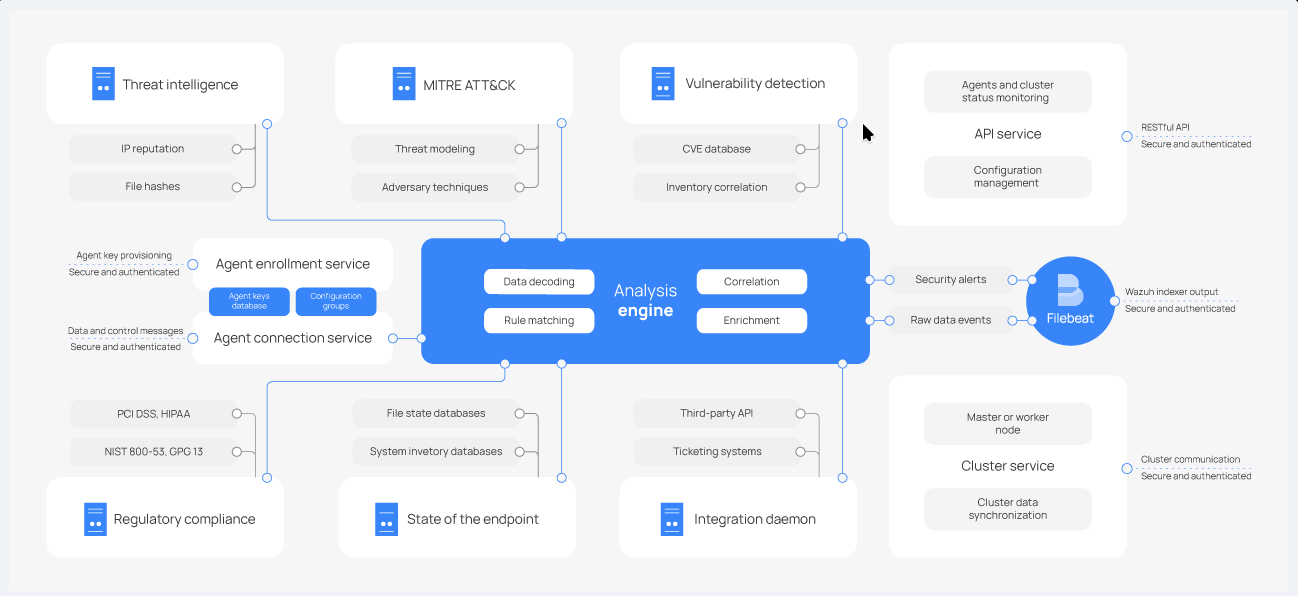
\includegraphics[width=0.9\textwidth]{figs/Wazuh_Server_Architecture.png}}
\caption{Wazuh Server Architecture}
\label{fig:Wazuh_Server_Architecture}
\end{figure}

\paragraph{2. Wazuh Server \cite{wazuh-server}}
\label{par:wazuh-server}

The Wazuh server examines agent data and generates alerts in case of threats. It helps manage agent configuration remotely and track their status. It uses threat intelligence and enriches alerts with frameworks like MITRE ATT\&CK and regulatory requirements.

The Wazuh server includes several components with specific functions: registration of new agents, validation of each agent's identity, encryption of communications between the Wazuh agent and the Wazuh server.
\begin{itemize}
    \item \textbf{Agent Registration Service:} Registers new agents and distributes unique authentication keys.
    \item \textbf{Agent Connection Service:} Verifies agent identity and manages centralized configurations.
    \item \textbf{Analysis Engine:} Analyzes data and detects patterns to trigger alerts.
    \item \textbf{Wazuh RESTful API:} Allows interaction with the Wazuh infrastructure and managing configurations and decoders.
    \item \textbf{Filebeat:} Sends events to the Wazuh server in real time.
\end{itemize}

\begin{figure}[H]
\centering
\fbox{
\includegraphics[width=0.8\textwidth]{figs/Division Systemes d'information.png}}
\caption{Organization Chart of the Information Systems Division}
\label{fig:organigramme_dsi}
\end{figure}

\paragraph{3. Wazuh Indexer \cite{wazuh-indexer}}
\label{par:wazuh-indexer}

The Wazuh indexer is a highly scalable full-text search and analysis engine. It is part of Wazuh and indexes server alerts, offering near real-time search and analysis. The indexer records data in JSON document format, linking various keys and values.

Wazuh uses four distinct indices for storing various types of events:
\begin{itemize}
    \item \textbf{wazuh-alerts:} Keeps alerts issued by the Wazuh server. These are generated each time an event activates a sufficiently high priority rule.
    \item \textbf{wazuh-archives:} Keeps all events received by the Wazuh server, whether they trigger a rule or not.
    \item \textbf{wazuh-monitoring:} Keeps information about agent status over time. The web interface uses it to show whether agents are active, disconnected, or have never been connected.
    \item \textbf{wazuh-statistics:} Keeps data related to Wazuh server performance. The web interface uses it to display performance statistics.
\end{itemize}

\paragraph{4. Wazuh Dashboard \cite{wazuh-dashboard}}
\label{par:wazuh-dashboard}

The Wazuh dashboard offers a flexible and intuitive web user interface. It allows exploring, analyzing, and visualizing security event and alert data. Furthermore, it constitutes an essential tool for managing and monitoring the Wazuh platform.
\begin{itemize}
    \item \textbf{Data Visualization and Analysis:} Allows exploring server data and security alerts, creating reports and custom visualizations.
    \item \textbf{Agent Monitoring and Configuration:} Users can manage and track agent status via the dashboard.
    \item \textbf{Platform Management:} Allows monitoring status, accessing logs, and configuring the Wazuh server.
    \item \textbf{Development Tools:} Includes a rule testing tool to verify message decoding from logs.
\end{itemize}


% ========== 3.6 SOAR CHOICE ==========
\section{SOAR Choice}
\label{sec:soar}

SOAR (Security Orchestration, Automation and Response) is an essential component of a Security Operations Center, designed to automate, orchestrate, and respond to security incidents. We chose platforms according to the three elements of SOAR which are SOA (Security Orchestration and Automation), SIRP (Security Incident Response Platform), and TIP (Threat Intelligence Platform).

\subsection{SOA: Shuffle}
\label{subsec:shuffle}

Shuffle was designed in response to several automation challenges requiring particular attention from the CERT/SIRT community. Automation solutions currently available in the security domain attempt to centralize numerous tasks: ticket management, indicator tracking, threat information processing, and much more, all on a single platform. Conversely, Shuffle's objective is to develop the most effective automation solution, while ensuring its compatibility with all existing tools \cite{shuffle-docs}.

\subsubsection{Architecture}
\label{subsubsec:shuffle-arch}

The platform is divided into two main parts: the server and the workers. The server hosts all components, from API activity to workflow validation, while workers are autonomous units operating similarly to microservices. The upper part (server) and the lower part (workers) can be installed on different hosts and clustered together \cite{shuffle-arch}.

\textbf{Single server installation:}

\begin{figure}[H]
\centering
\fbox{\parbox{0.8\textwidth}{\centering\vspace{2cm}\textit{Figure 3.4 -- Shuffle Architecture}\vspace{2cm}}}
\caption{Shuffle Architecture}
\label{fig:shuffle-arch}
\end{figure}

\paragraph{1. Frontend (Graphical User Interface)}
\label{par:shuffle-frontend}

The frontend is developed in ReactJS, offering an intuitive user interface for:
\begin{itemize}
    \item Creating and managing workflows via a drag-and-drop interface.
    \item Visualizing workflow execution in real time.
    \item Managing users, organizations, and applications.
\end{itemize}

It uses libraries such as Cytoscape for workflow graphical representation and Material UI for interface components.

\paragraph{2. Backend (Main Server)}
\label{par:shuffle-backend}

The backend, developed in Go (Golang), is responsible for:
\begin{itemize}
    \item Managing secure REST APIs.
    \item Validating, storing, and scheduling workflows.
    \item Managing users, organizations, and access rights.
    \item Communication with other components such as Orborus and Workers.
\end{itemize}

It constitutes the heart of the platform, orchestrating all operations.

\subsubsection{Datastore (Database)}

Shuffle uses OpenSearch, a NoSQL database, to store:
\begin{itemize}
    \item Workflow definitions.
    \item Application configurations.
    \item Execution metadata.
    \item Information on users and organizations.
\end{itemize}

This database ensures the persistence of data essential to the platform's operation.

\subsubsection{Orborus (Worker Scheduler)}

Orborus is a component written in Go that acts as a scheduler for Workers. Its responsibilities include:

\begin{itemize}
    \item Deployment and management of Workers.
    \item Monitoring Worker status (active, inactive).
    \item Distributing workflow execution tasks to appropriate Workers.
\end{itemize}

It ensures efficient orchestration and optimal workload distribution.

\subsubsection{Workers (Execution Units)}

Workers are autonomous execution units that process actions defined in workflows. Their main characteristics are:

\begin{itemize}
    \item Execution of specific tasks (API calls, data processing, etc.).
    \item Parallel operation for horizontal scalability.
    \item Deployment on separate hosts for geographic distribution or task isolation.
\end{itemize}

They enable distributed and efficient workflow execution.

\subsubsection{Applications (Apps)}

Apps are integration modules that allow Shuffle to interact with external tools and services. Their characteristics include:

\begin{itemize}
    \item Development in Python or configuration via an \texttt{appspec.yaml} file.
    \item Each App groups several actions, representing specific operations (e.g., send a Slack message, create an alert in TheHive, make an API request).
    \item Apps are executed by Workers and can be shared or customized.
    \item Users can create their own Apps via a dedicated interface or by cloning existing templates from the official Shuffle GitHub repository.
\end{itemize}

\textbf{Note:} Before use in a workflow, an App must be activated and possibly configured with API credentials or environment parameters.

\subsubsection{Workflows}

Workflows are directed graphs representing task automation. They are the central element of Shuffle and allow a series of actions to be executed automatically. Their operation is as follows:

\begin{itemize}
    \item Created via a visual interface (drag-and-drop) or via API.
    \item Composed of nodes (actions) logically connected.
    \item Can include:
    \begin{itemize}
        \item Conditions (if/else),
        \item Loops,
        \item Variables (global or local),
        \item Custom API calls.
    \end{itemize}
    \item Workflows are versioned and can be tested manually or triggered automatically.
\end{itemize}

Each execution of a workflow is called a \textbf{run}, and can be consulted in real time to view errors or results of each step.

\subsubsection{Triggers}

Triggers serve to automatically start a workflow based on an event. They are entry points defined by the user or by an integration. Main types:

\begin{itemize}
    \item \textbf{HTTP Triggers (Webhooks):} Receive external requests (e.g., from a SIEM or a security alert).
    \item \textbf{Scheduled Triggers:} Scheduled execution via cron-type rules (e.g., every hour, every Monday).
    \item \textbf{App Triggers:} Execution triggered by certain Apps or integrations.
\end{itemize}

Each trigger can pass input parameters to the workflow, usable as variables in subsequent steps.

% ========== 3.6.2 SIRP: TheHive ==========
\subsection{SIRP: TheHive}
\label{subsec:thehive}

TheHive offers a comprehensive "4-in-1" security incident response platform, constituting an essential tool for SOCs, CSIRT Teams, CERT Teams, as well as all cybersecurity professionals involved in rapid and effective incident management.

It brings together a robust set of features designed to optimize incident response workflows, strengthen collaboration, and enable security analysts to conduct in-depth investigations and effectively contain threats.

Thanks to its seamless integration with MISP and its advanced capabilities in task management, evidence processing, and threat intelligence integration, TheHive stands out as an indispensable tool for modern SOC, CSIRT, and CERT teams \cite{thehive-docs}.

\subsubsection{Key Features}

\begin{itemize}
    \item \textbf{Integration with MISP:} Close integration with MISP for seamless collaboration and effective information sharing.
    \item \textbf{Real-time Collaboration:} Multiple analysts can collaborate simultaneously thanks to live updates on cases, tasks, observables, and Indicators of Compromise (IOCs).
    \item \textbf{Efficient Task Management:} Dedicated notifications allow efficient task management and assignment, with the ability to import data from various sources such as email reports, CTI providers, and SIEMs.
    \item \textbf{Customizable Templates:} Creation of cases and tasks using a flexible template engine, allowing the addition of custom metrics and fields to drive team activity and identify automation opportunities.
    \item \textbf{Evidence Management:} Analysts can record their progress, attach evidence or files, add tags, and securely import password-protected ZIP archives containing suspicious data.
    \item \textbf{Observable Management:} Easy addition and management of observables, individually or in bulk, with the ability to import directly from MISP events or alerts. Sorting and filtering functions facilitate processing.
    \item \textbf{Threat Intelligence Integration:} Use of analyzers and responders to enrich investigations, accelerate detection, and contain threats. Use of tags, IOC reporting, and recognition of previously encountered observables to strengthen cyber intelligence.
\end{itemize}

\subsubsection{Architecture}

TheHive can be installed on a single server or in a cluster according to scalability needs. Its modular architecture allows deploying the application, database, indexing engine, and file storage separately, offering flexibility and scalability.

The key components are:
\begin{itemize}
    \item \textbf{Apache Cassandra:} For data storage,
    \item \textbf{Elasticsearch:} For indexing,
    \item \textbf{File Storage:} Via local file system, NFS, or S3 MinIO depending on the environment.
\end{itemize}

\paragraph{1. TheHive (Main Application)}

TheHive is the heart of the platform, offering an intuitive web interface for security incident management. It allows analysts to create, track, and collaborate on cases, and to analyze observables. The application is designed to be deployed in standalone mode or in cluster, thus ensuring high availability and scalability adapted to organizational needs.

\paragraph{2. Apache Cassandra (Database)}

Apache Cassandra is a distributed NoSQL database used by TheHive to reliably store information relating to cases, tasks, observables, and other entities. Its design without a single point of failure ensures high availability and fault tolerance. In a cluster configuration, it is recommended to deploy at least three Cassandra nodes with a replication factor of 3 to guarantee data redundancy.

\begin{figure}[H]
\centering
\fbox{\parbox{0.8\textwidth}{\centering\vspace{2cm}\textit{Figure 3.5 -- Cassandra}\vspace{2cm}}}
\caption{Cassandra}
\label{fig:cassandra}
\end{figure}

\paragraph{3. Elasticsearch (Indexing Engine)}

Elasticsearch is used to quickly index and search data stored in TheHive. It enables efficient searches on cases, observables, and other entities, thus facilitating information analysis and correlation. TheHive is compatible with versions 7.x and 8.x of Elasticsearch. It is also possible to use OpenSearch as an alternative.

\begin{figure}[H]
\centering
\fbox{\parbox{0.8\textwidth}{\centering\vspace{2cm}\textit{Figure 3.6 -- Elasticsearch}\vspace{2cm}}}
\caption{Elasticsearch}
\label{fig:elasticsearch}
\end{figure}

\paragraph{4. MinIO (Object Storage)}

MinIO is an S3 API-compatible object storage solution used by TheHive to store files associated with cases, such as attachments, evidence, and reports. It offers horizontal scalability and high availability, essential for clustered environments. Each TheHive node can be configured to access MinIO via a load balancer, thus ensuring efficient file distribution.

\begin{figure}[H]
\centering
\fbox{\parbox{0.8\textwidth}{\centering\vspace{2cm}\textit{Figure 3.7 -- MinIO}\vspace{2cm}}}
\caption{MinIO}
\label{fig:minio}
\end{figure}

% ========== 3.6.3 TIP ==========
\subsection{TIP: Threat Intelligence Platform}
\label{subsec:tip}

In a SOAR architecture, the integration of Threat Intelligence services through public APIs constitutes an essential element of enrichment process automation. Platforms such as VirusTotal, AbuseIPDB, or IPinfo allow rapid acquisition of contextual information on suspicious files, IP addresses, or domains. These APIs are used to feed analysis workflows, facilitate automated decision-making, and improve the quality of security incident responses.

\subsubsection{VirusTotal}

VirusTotal is a file and URL analysis service that relies on more than 70 antivirus engines as well as URL and domain blocklisting services. It also uses various tools to extract indicators from analyzed content. Any user can submit a file via a web interface accessible from a browser. Several submission methods are offered: the public web interface (priority in the queue), desktop applications, browser extensions, as well as a programmatic API. This API, based on HTTP, allows automating file submissions from any programming language.


\subsubsection{EmailRep}

EmailRep is a system composed of crawlers, scanners, and enrichment services, designed to collect data on email addresses, domain names, and digital identities across the Internet. It relies on hundreds of information sources, including social media profiles, professional networking sites, dark web credential leaks, data breaches, phishing kits, malicious emails, spam lists, open mail relays, as well as data on domain age and reputation or email deliverability. These elements are analyzed to assess the risk level associated with an email address.

% ========== 3.7 LOAD BALANCER ==========
\section{Load Balancer}
\label{sec:loadbalancer}

A load balancer consists of distributing computing workload across multiple computers. On the Internet, this approach is frequently used to distribute network traffic across multiple servers. This reduces the load on each server, thus increasing their efficiency, accelerating performance, and reducing latency \cite{loadbalancer}.

\subsection{HAProxy}
\label{subsec:haproxy}

HAProxy (High Availability Proxy) is an open-source load balancer renowned for its performance, reliability, and flexibility, supporting both TCP and HTTP/HTTPS layers \cite{haproxy-docs}.

\subsubsection{Characteristics of HAProxy}

\begin{enumerate}
    \item \textbf{High Performance:} Handles a large number of requests per second with minimal latency, optimized for modern architectures (microservices, cloud).

    \item \textbf{Distribution Algorithms:}
    \begin{itemize}
        \item \textbf{Round Robin:} Cyclic distribution of requests.
        \item \textbf{Least Connections:} Prioritizes the least busy servers.
        \item \textbf{Source IP Hash:} Session persistence based on client IP.
    \end{itemize}

    \item \textbf{Health Checking:} Verifies backend server availability via HTTP/TCP requests.

    \item \textbf{Security:} Protection against DDoS attacks using ACLs and rate limiting.
\end{enumerate}

\begin{figure}[H]
\centering
\fbox{\parbox{0.8\textwidth}{\centering\vspace{2cm}\textit{Figure 3.8 -- Load Balancer}\vspace{2cm}}}
\caption{Load Balancer}
\label{fig:loadbalancer}
\end{figure}

% ========== 3.8 SOC PLATFORM OPERATION ==========
\section{Operation of the SOC Platform}
\label{sec:operation}

We present below the operation of our SOC solution.

\begin{enumerate}
    \item \textbf{Data/Log Collection:} Comprehensive data collection is performed from various sources, including operating systems, network equipment, cloud applications, databases, and security tools. Logs are centralized via lightweight agents and standardized protocols, ensuring total visibility of the IT infrastructure, on-premises or in the cloud.

    \item \textbf{Indexing and Storage:} Once data is collected, it is normalized and indexed in a database (Wazuh Indexer) for rapid searches. Retention policies of 30 to 90 days are implemented to comply with legal and operational requirements.

    \item \textbf{Data Analysis:} Custom queries help recognize attack patterns within the MITRE ATT\&CK framework, such as lateral movement or data exfiltration. For example, multiple login failures followed by a success trigger an analysis to detect potential compromise.

    \item \textbf{Alert Triggering:} Detected anomalies generate alerts that are classified according to their criticality level, ranging from low to critical. These alerts are accompanied by contextual metadata, such as the source IP address and the concerned user, before being transmitted to our SOAR platform.

    \item \textbf{Alert Triage:} Alerts are carefully filtered to remove false positives and prioritize real threats. SOC analysts rely on interactive dashboards to visualize the history of similar incidents and assess their degree of urgency.

    \item \textbf{Observable Extraction:} This step consists of identifying important Indicators of Compromise (IOCs), such as IP addresses, file hashes, suspicious URLs, or abnormal behaviors.

    \item \textbf{Observable Analysis and Enrichment:} IOCs are enriched via Threat Intelligence sources to assess their reputation and their relationship with known campaigns. A file hash can be verified in malware databases to validate its dangerousness. Enrichment also includes correlation with previous incidents: an IP linked to a DDoS attack will be considered with higher priority.

    \item \textbf{Execution of Appropriate Playbooks:} Once the threat is characterized, predefined playbooks, adapted to the identified risk type, are activated to orchestrate the response.
\end{enumerate}

\begin{figure}[H]
\centering
\fbox{\parbox{0.8\textwidth}{\centering\vspace{2cm}\textit{Figure 3.9 -- SOC Platform Operation}\vspace{2cm}}}
\caption{SOC Platform Operation}
\label{fig:soc-operation}
\end{figure}

% ========== 3.9 CONCLUSION ==========
\section{Conclusion}
\label{sec:conclusion}

This chapter presented the detailed analysis and design of our SOC-as-a-Service platform, highlighting the essential criteria that guided the choice of tools as well as their integration within a scalable and secure architecture. We opted for open-source solutions such as Wazuh (SIEM/XDR) and Shuffle (SOAR), combined with TheHive for incident management, to meet the requirements of detection, analysis, and response to threats. In conclusion, this robust design, coupled with interoperable tools adapted to the needs of SMEs, lays the foundations for an effective SOC, capable of adapting to the evolutions of the cyber landscape. The next steps will consist of implementing this architecture and evaluating its performance in an operational environment, as detailed in the next chapter.

% ========== BIBLIOGRAPHY ==========
\begin{thebibliography}{99}
\bibitem{k8s-docs} Kubernetes Documentation, \textit{Kubernetes Components}, available at: \url{https://kubernetes.io/docs/concepts/overview/components/}
\bibitem{helm-docs} Helm Documentation, \textit{Helm -- The package manager for Kubernetes}, available at: \url{https://helm.sh/docs/}
\bibitem{wazuh-community} Wazuh, \textit{Wazuh Community}, available at: \url{https://wazuh.com/community/}
\bibitem{wazuh-agent} Wazuh Documentation, \textit{Wazuh Agent}, available at: \url{https://documentation.wazuh.com/current/installation-guide/wazuh-agent/index.html}
\bibitem{wazuh-server} Wazuh Documentation, \textit{Wazuh Server}, available at: \url{https://documentation.wazuh.com/current/installation-guide/wazuh-server/index.html}
\bibitem{wazuh-indexer} Wazuh Documentation, \textit{Wazuh Indexer}, available at: \url{https://documentation.wazuh.com/current/installation-guide/wazuh-indexer/index.html}
\bibitem{wazuh-dashboard} Wazuh Documentation, \textit{Wazuh Dashboard}, available at: \url{https://documentation.wazuh.com/current/installation-guide/wazuh-dashboard/index.html}
\bibitem{shuffle-docs} Shuffle, \textit{Shuffle Documentation}, available at: \url{https://shuffler.io/docs/about}
\bibitem{shuffle-arch} Shuffle, \textit{Shuffle Architecture}, available at: \url{https://shuffler.io/docs/architecture}
\bibitem{thehive-docs} TheHive Documentation, \textit{TheHive - Security Incident Response Platform}, available at: \url{https://docs.thehive-project.org/}
\bibitem{loadbalancer} Load Balancer Definition, available at: \url{https://en.wikipedia.org/wiki/Load_balancing_(computing)}
\bibitem{haproxy-docs} HAProxy Documentation, \textit{HAProxy - The Reliable, High Performance TCP/HTTP Load Balancer}, available at: \url{https://www.haproxy.org/}
\end{thebibliography}